\setcounter{page}{1}
\setcounter{equation}{0}
\setcounter{figure}{0}
\setcounter{table}{0}

\section{Introduction}

- Popisat o com je process control (vo vseobecnosti)
- Popisat v strucnosti ako sa vyvija kybernetika
- Popisat v strucnosti ako sa vyvija automatizacia
- Spomenut nove trendy - Industry 4.0, IoT, Industrial IoT, Edge computing
- Softverova podpora process control a kybernetiky na baze AI, deep learning a machine learning - ake metody, ake modely, co sa pouziva u nas na ustave

-----------------

The objective of process control is to keep key process-operating parameters within narrow bounds of the reference value or setpoint. This chapter describes the theory behind control circuits to maintain automatic control over a process. The basis of automatic control is the control loop. A control loop for a given process must have at least one sensor, a controller, and a control element to which the results are applied. A good example of automatic control is electric heating of a house in a cold environment, a process where a single variable is controlled. A thermostat (sensor) monitors the temperature. When the temperature drops below the setpoint, a switch is closed and the heater comes on. When the temperature rises above the setpoint, the switch opens and the heater is turned off. The difference between the actual value and the setpoint is called the error. The controller reads the error and makes a decision. The action taken can be very simple to very complicated, depending on the system and the size of the acceptable error.

Process industries have developed along similar lines with control systems. To answer the question of what process control is exactly, we have to go back to the earliest introductions of control mechanisms, where first-generation electro-pneumatic-mechanical loop controllers replaced people doing tasks such as manually adjusting valves in response to some local indicator like a pressure gauge.



Although a device was used to automate a human function in an effort to control a variable, there was no sense of what the process was doing overall. A basic controller could keep an individual loop on an even keel, more or less, so long as there was not too much disruption. Complex processes might employ dozens or even hundreds of such controllers, each with its performance displayed on a panel board, but keeping an eye on the big picture was still a human process.


When distributed control system (DCS) platforms were introduced in the 1970s, they simplified the mechanics of the panel board, but did not do much to improve its capabilities. Big-picture analysis was still largely a human responsibility. Sure, getting beyond the technical constraints of pneumatic field devices with their troublesome compressed air tubing made it easier to install more instruments and actuators, but the basic control concepts did not really change. Any movement to advanced process control (APC) and other forms of control optimization were still in their infancy. Process automation capable of supporting APC had to encompass many technologies and techniques. It was characterized by incorporating many more input data points into algorithms and orchestrating more complex sequences.


The transition to process automation and APC was empowered by being able to create an all-encompassing platform capable of coordinating more than single loops or small cascade groups. One major advantage of newer platforms is the ability to optimize a process to suit the owner’s specific economic goals based on any number of desired outcomes. The process automation system can operate the plant to minimize energy consumption, maximize output, and deliver specific product quality attributes.

Implementing such systems is challenging. During the initial design phase of a control system upgrade or a new installation, it is far too easy to focus just on process fundamentals, and never get beyond considering desired steady-state conditions. Automation system upgrades and new installations can therefore miss opportunities to engage with process and automation technology experts capable of uncovering better ways of doing things.

Many capabilities of modern process automation systems are still underutilized in most process plants, even among companies most people would consider sophisticated. Far fewer companies use APC as effectively as they could, even though basic APC technologies have been around for decades. -------- Even the most modern process plants typically do not take full advantage of the capabilities of their control systems. ------------------

Peter Drucker, a well-known management thinker, who has been quoted multiple times over the years by various people, has famously said: “If you can't measure it, you can't manage it. If you can't manage it, you can't improve it.” His words are now resonating more than ever with the push towards Industry 4.0.

Big Data means the analysis of large amounts of data coming from different sources with high speed and with the aim to create economic benefit.

-----------------------------


The oxygen converter process (LD/BOF and its derivatives) is a refinement step in the production of steel from ore. The main purpose of the process is to remove excess carbon from the pig iron produced in the blast furnace. The main feature of the process is to add oxygen through a top lance, in order to remove unwanted impurities through oxidation. It is the main method of carbon and low alloy steelmaking, annual production approaching to 60\% of total crude steel production \citep{Jalkanen2006}. BOF is a widely preferred and effective steelmaking method due to its high productivity and considerably low production cost \citep{Wang2010}.

 LD/BOF process consists of these subprocesses:

\begin{enumerate}
	\item Charging slag
	\item Charging hot metal 
	\item Oxygen blowing and addition of slagging and alloying additives
	\item Measurement of steel temperature and composition
	\item Tapping of steel
	\item Tapping of slag
\end{enumerate}

The first commercial operation of steelmaking with oxygen top blowing in the converter was in the early 1950s at Linz and Donawitz (Austria). This manner of steelmaking became known as Linz-Donawitz or LD process. For many years now, most of the steel has been made by top oxygen blowing for which different names are given. For example, in European steel plants the process is still called LD; in the UK, BOS (basic oxygen steelmaking); in the Far East and America, BOF (basic oxygen furnace), with the exception of U.S. Steel where it is called BOP (basic oxygen process) \citep{Turkdogan1996}.

\begin{figure}[h!]
	\centering
	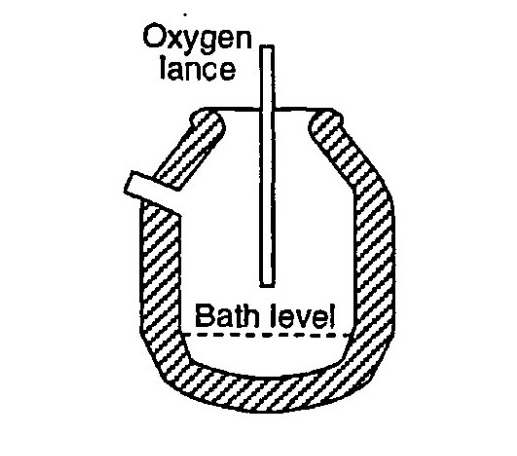
\includegraphics[width=.5\textwidth,angle=0]{bof-single.jpg}
	\caption{Production of steel in the converter with top-blown oxygen (LD/BOF) \citep{Turkdogan1996}.}
	\label{o:1}
\end{figure}

In the early 1970s, a bottom-blown oxygen steelmaking process was developed in Canada and Germany. This process, known as OBM in Europe and Q-BOP elsewhere, was in full size commercial operation by the mid 1970s in U.S. Steel plants followed by several plants in Europe and Japan. The tuyeres, mounted in a removable bottom, consist of a central pipe for blowing oxygen together with burnt lime, and an annular gap around the central pipe for the passage of gaseous hydrocarbon, e.g. propane or natural gas \citep{Turkdogan1996}.

\begin{figure}[h!]
	\centering
	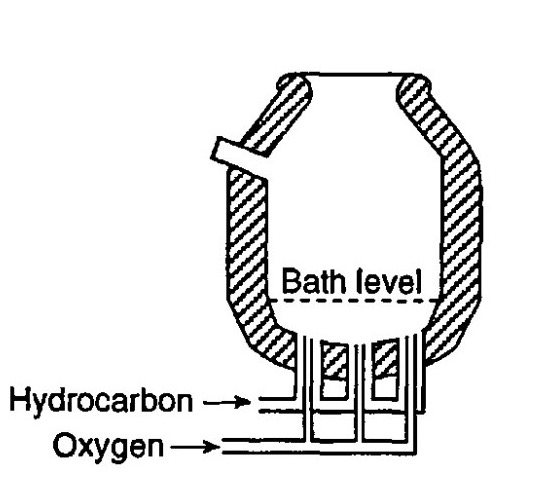
\includegraphics[width=.5\textwidth,angle=0]{q-bop.jpg}
	\caption{Production of steel in the converter with bottom-blown oxygen (Q-BOP) \citep{Turkdogan1996}.}
	\label{o:2}
\end{figure}

Further developments in oxygen steelmaking led to the present practices of various types of top and bottom blowing known as combined blowing, as illustrated schematically in Fig. 8.1 for BOF and Q-BOP processes. There is also post combustion of CO in the upper part of the vessel to generate additional heat for steelmaking \citep{Turkdogan1996}.

\begin{figure}[h!tbp]
	\centering
	\subfloat[Combined LD/BOF.]{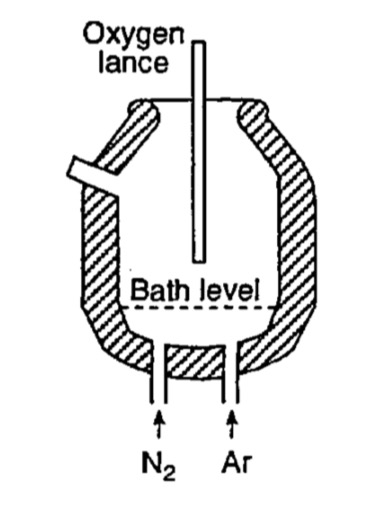
\includegraphics[width=0.38\textwidth]{kombinovany-bof.jpg}\label{fig:f1}}
	\hfill
	\subfloat[Combined Q-BOP.]{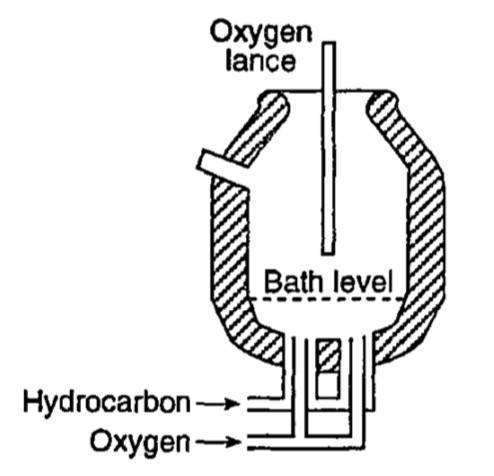
\includegraphics[width=0.52\textwidth]{kombinovany-q-bop.jpg}\label{fig:f2}}
	\caption{LD/BOF a Q-BOP processes in oxygen convertor with combined blowing.}
	\label{o:3}
\end{figure}

In modern steel mills about 300 tons of steel are produced within a 30-40 minute cycle. Various additives are added during the process to adapt the steel quality and slag formation. The converter furnace is inclined during charging and tapping. The converter has a vertical position during oxygen blowing. The changes in the position of the converter during the individual elementary processes are shown in the figure \ref{o:4}.

\begin{figure}[h!]
	\centering
	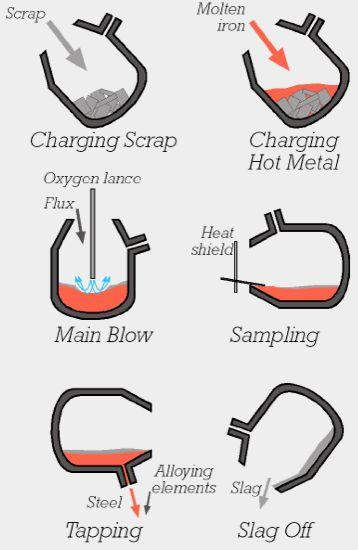
\includegraphics[width=.45\textwidth,angle=0]{convertor-phases.jpg}
	\caption{Representation of elementary processes in LD converter.}
	\label{o:4}
\end{figure}

Depending on local operating conditions, availability of scrap, blast furnace iron and the extent of hot metal pretreatment, the metallic charge (LD/BOF, Q-BOP) is 75 to 95 \% pig iron and the remainder is steel scrap. The types of scrap used are usually those produced in a steel mill: sheet scrap, damaged molds, bimetallic cans etc \cite{Turkdogan1996}.

Oxygen is blown at a high speed (up to twice the speed of sound) on the surface of the metal bath in the converter and so-called hot area is formed in the region where the oxygen stream hits the surface. The oxidation products dissolve in the slag, with the exception of carbon monoxide, which passes through the slag layer and forms the major component of the converted gas. The oxidation intensity of the individual elements depends on their chemical affinity for oxygen. Carbon oxidation is one of the most important processes. Carbon is oxidized in the metal during the steelmaking process by the influence of oxygen, in particular on \ce{CO} and~partly on \ce{CO2}, depending on the reactions

\begin{equation}
\ce{C + 1/2O2 -> CO}
\end{equation}
\begin{equation}
\ce{C + O2 -> CO2}
\end{equation}

Manganese is oxidized to \ce{MnO}

\begin{equation}
\ce{Mn + 1/2O2 -> MnO}
\end{equation}

Phosphorus is undesirable in steel and oxidizes to \ce{P2O5}

\begin{equation}
\ce{2P + 5/2O2 -> P2O5}
\end{equation}

Sulphur is a harmful element and passes into the slag in the form of \ce{CaS} based on the reaction of \ce{CaO}

\begin{equation}
\ce{CaO + MnS -> CaS + MnO}
\end{equation}

whereby \ce{MnS} is formed by reaction

\begin{equation}
\ce{Mn + S -> MnS}
\end{equation}

and sulphur also goes out in the form of gas as \ce{SO2}

\begin{equation}
\ce{S + O2 -> SO2}
\end{equation}

Silicon has a high affinity for oxygen, so it is easily oxidized to form \ce{SiO2}

\begin{equation}
\ce{Si + O2 -> SiO2}
\end{equation}

In the initial stages of blowing, most of the silicon oxidizes to form a slag of low basicity - the composition of the metal and slag changes, as shown in the figure \ref{o:20}.

\begin{figure}[h!]
	\centering
	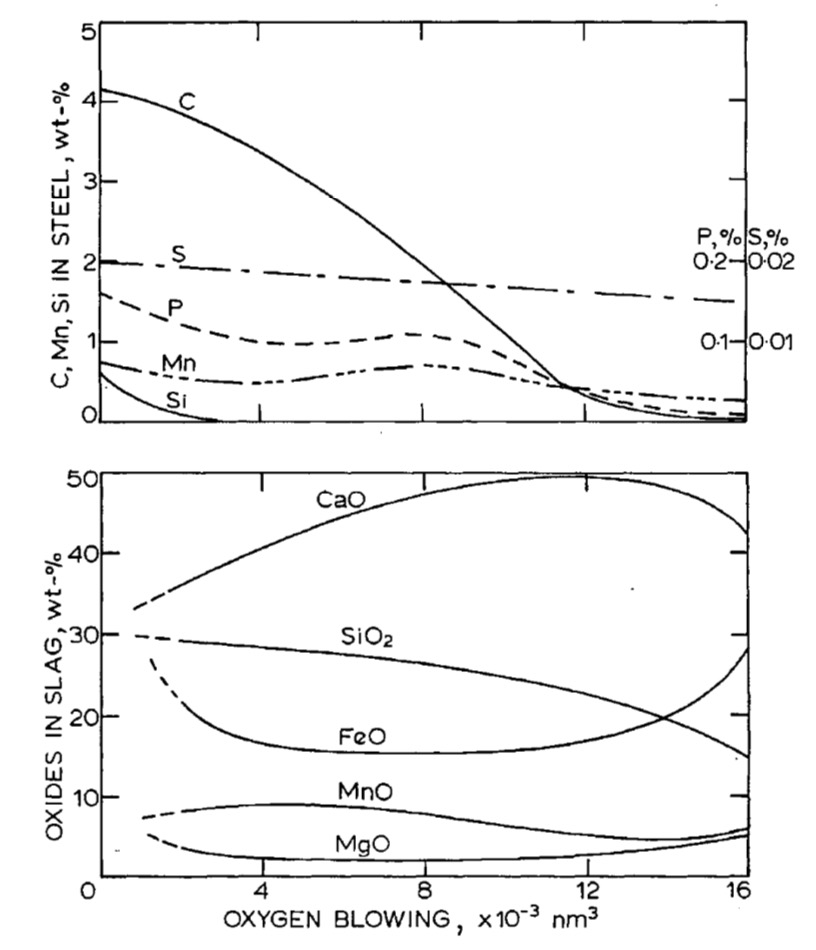
\includegraphics[width=.51\textwidth,angle=0]{slag-formation-data.jpg}
	\caption{Changes in metal and slag composition during steel production in LD/BOF process \citep{Turkdogan1996}.}
	\label{o:20}
\end{figure}

An intense oxygen flow induces fluid flows in the iron bath, forcing the highly oxidized metal and the molten oxidation products from the iron bath surface to penetrate into the bath, where they react with the "fresh" hot metal with a high content of impurities and therefore loss of iron in the form of \ce{FeO} and~\ce{Fe2O3} should also be considered:

\begin{equation}
\ce{Fe + 1/2O2 -> FeO}
\end{equation}

\begin{equation}
\ce{2Fe + 3/2O2 -> Fe2O3}
\end{equation}.

This oxygen stream and gas bubbles generated in the bath bring portions of the iron melt to the slag. The heat generated by the highly exothermic oxidation reactions is consumed by heating and melting the feed materials, heating the iron bath, slag and carbon oxides that are formed during the oxidation of the carbon and are partially lost to the environment during the blowing process.

The resulting \ce{SiO2} passes into the slag as \ce{2CaO.SiO2} according to the equation

\begin{equation}
\ce{SiO2 + 2CaO -> 2CaO.SiO2}
\end{equation}

and additionally, \ce{P2O5} passes into the slag as \ce{3CaO.P2O5} according to the equation \cite{sprava2017}

\begin{equation}
\ce{P2O5 + 3CaO = 3CaO.P2O5}.
\end{equation}

Circulation in the iron bath caused by the flow of oxygen, rising gas bubbles and purging of inert gas through the lower tubes in converters with combined blowing type transports minor iron melt components (C, Si, Ti, Mn, P, V, etc.) to the upper bath layers \cite{Jalkanen2006}. 

\begin{figure}[h!]
	\centering
	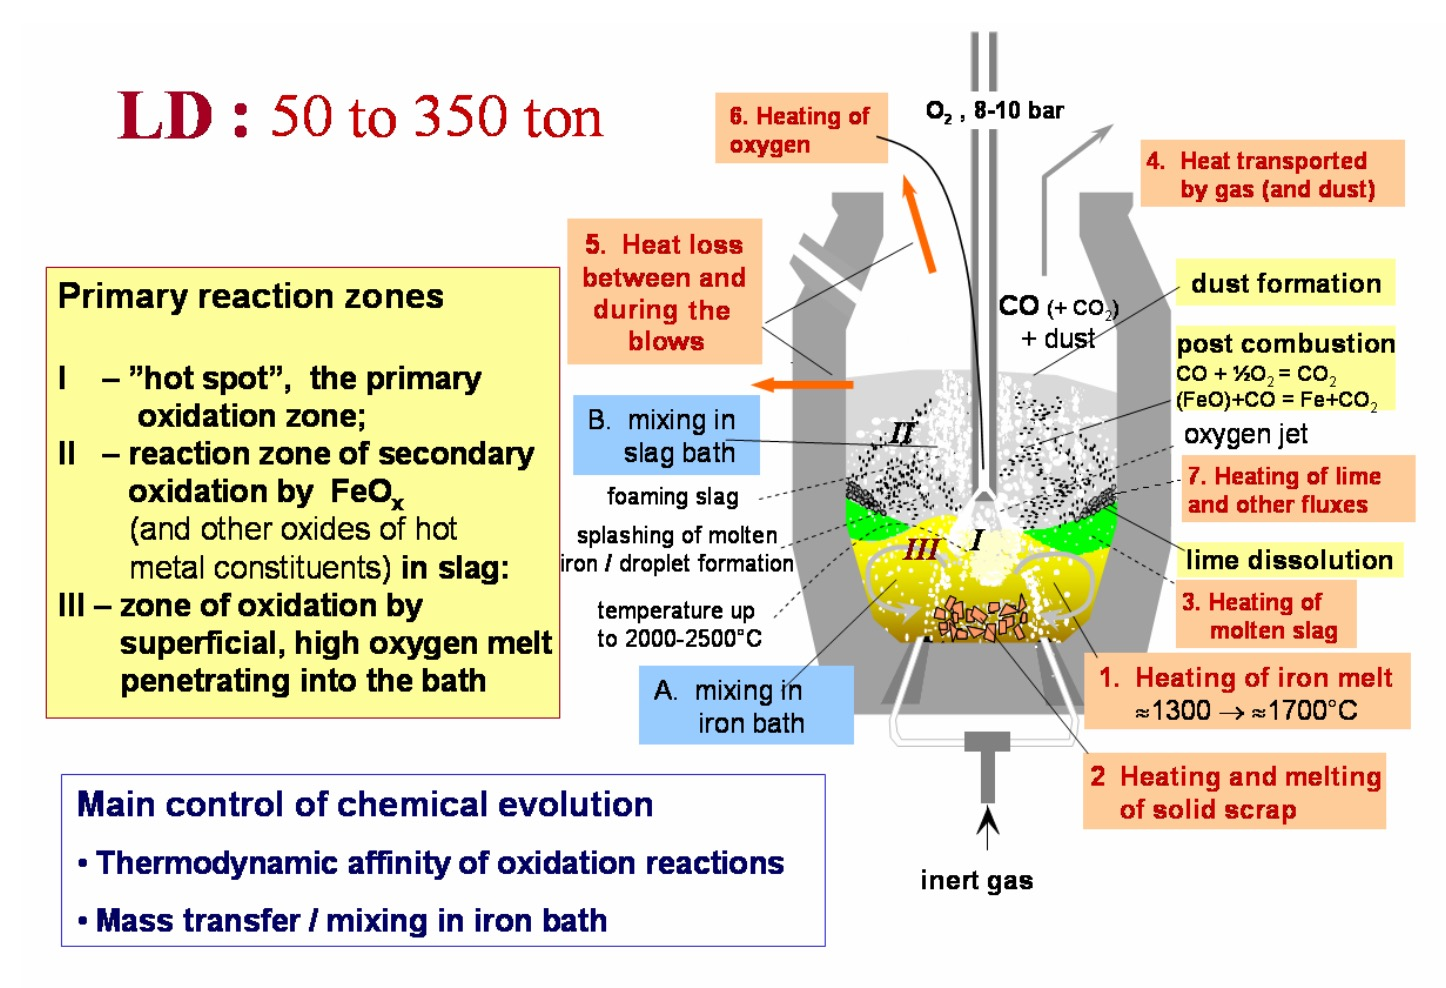
\includegraphics[width=.9\textwidth,angle=0]{ld-convertor-processes-graphical.jpg}
	\caption{Chemical and thermal processes in LD converter \citep{Jalkanen2006}.}
	\label{o:25}
\end{figure}

\begin{figure}[h!]
	\centering
	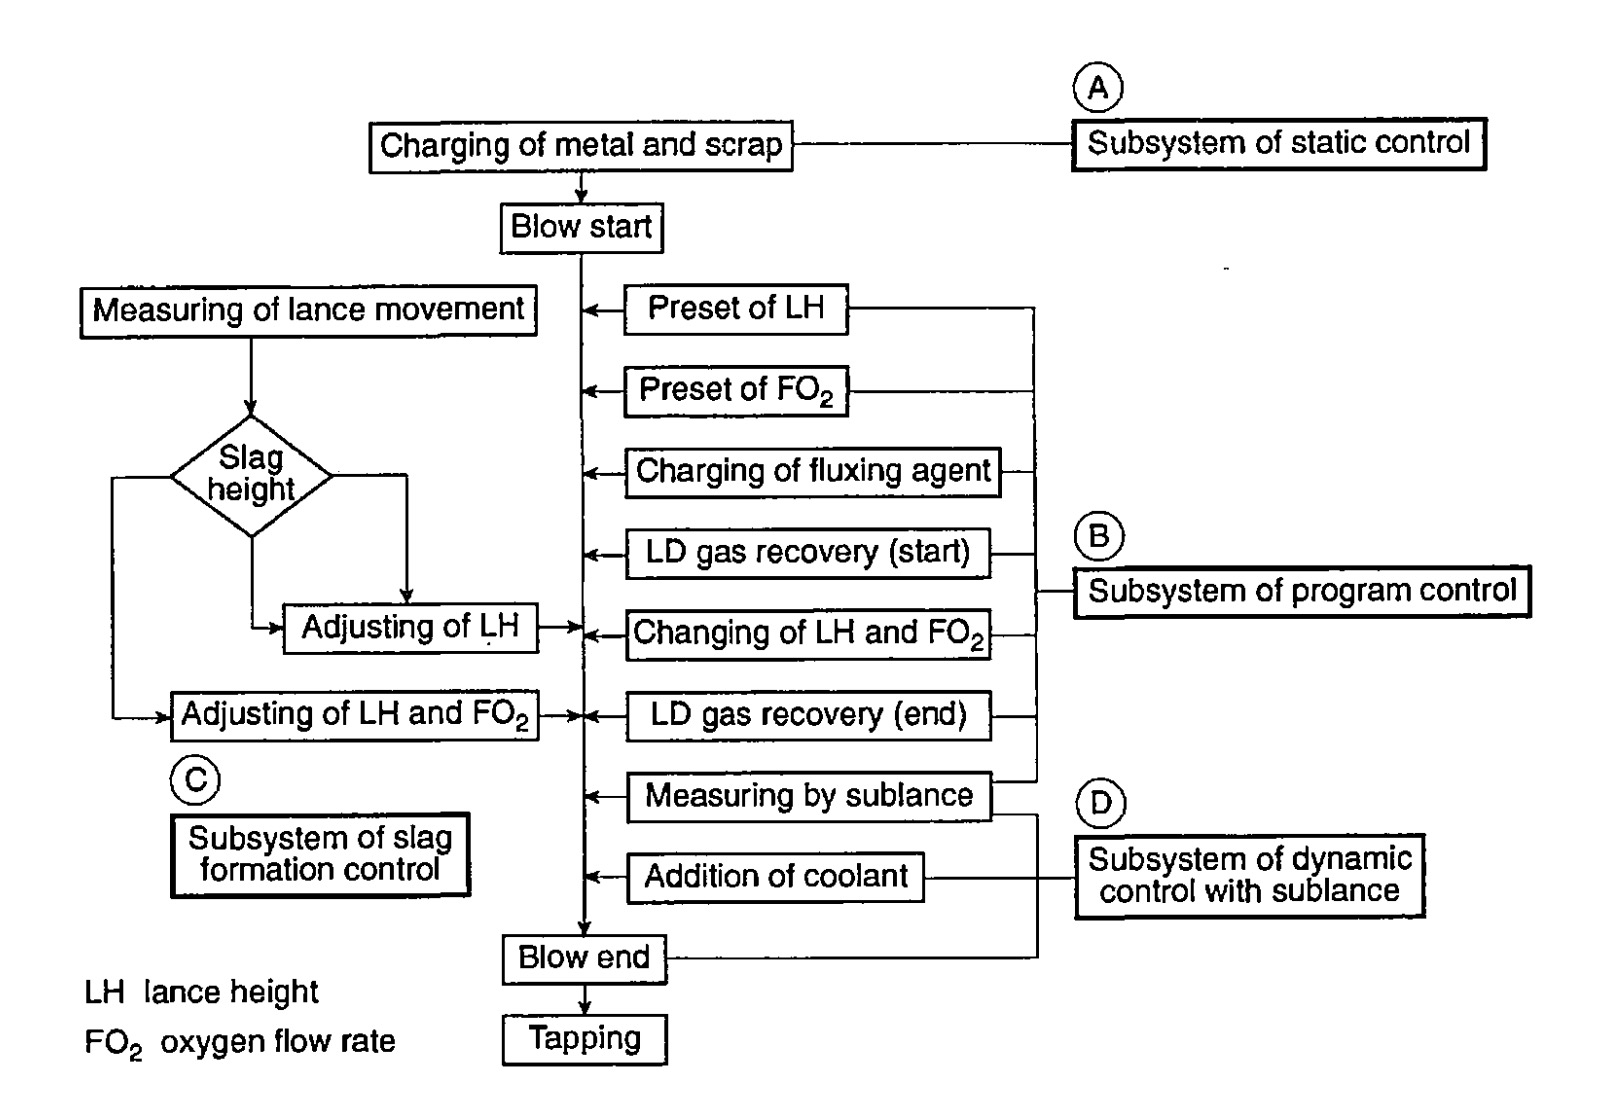
\includegraphics[width=.8\textwidth,angle=0]{control-schematic-bof.jpg}
	\caption{Schematic representation of the system and function of fully automatic LD/BOF process \citep{Turkdogan1996}.}
	\label{o:i31}
\end{figure}